\subsection{DK-kogebogen}
DK-Kogebogen er en web-applikation, som tilbyder en lang række funktioner, hvoraf ``Tøm køleskabet'' er en af dem. Udover ``tøm køleskabet'', tilbyder DK-kogebogen også en ugentlig madplan, en ekstern hjemmeside med fokus på viden omkring mad (energiindhold, vitaminindhold osv.), en kalorieberegner og meget meget mere. Sagt med andre ord, så prioriterer DK-Kogebogen ikke udelukkende sine ressourcer på ``Tøm køleskabet'', og dette kan påvirke kvaliteten af denne. Desuden kan det også være svært at skabe sig et overblik på hjemmesiden, da der er så mange funktioner pakket sammen på samme side. Siden har et omfang af 36.434 opskrifter, hvilket er det klart største antal blandt de undersøgte forbilleder. De mange opskrifter er indsendt og lavet af brugere af hjemmesiden. Dette kan både være positivt og negativt. Det kan være negativt, da der kan forekomme en del fejl i opskrifterne. DK-Kogebogen skriver på deres hjemmeside, om de indsendte opskrifter:

%kilde: http://www.dk-kogebogen.dk/opskrifts-service/indsend-opskrift.php
\begin{quote}
``Opskriften kan ses med det samme, men der vil senere blive rettet lidt til i teksterne.''
\end{quote}

Altså er det muligt for alle og enhver at indsende opskrifter, som er fulde af fejl, og disse vil alligevel være synlige på siden. Til gengæld skaber den mulighed, der ligger i at brugerne kan indsende deres egne opskrifter,\tjek{[Giver denne sætning mening?]} at den enkelte bruger føler sig mere knyttet til siden, da han/hun har et personligt engagement i den; og dette vil resultere i en overordnet højere brugeraktivitet. Det skal noteres, at de 36.434 opskrifter ikke er unikke. Det vil sige, at der godt kan eksistere flere forskellige varianter af den samme opskrift; \fx er der 17 forskellige varianter af Boller i Karry, hvilket kan virke uoverskueligt.

Når brugeren vil anvende ``Tøm køleskabs''-funktionen, mødes vedkommende af følgende billede \ref{fig:dk-kogebogen1}, som er et udklip fra toppen af DK-Kogebogens forside. Her kan brugeren indtaste så mange ingredienser han/hun har lyst til, inden for en grænse på 55 karakter. For at systemet kan identificere ingredienser, skal der mellem hver ingrediens, som brugeren indtaster, være et mellemrumstegn. Begrænsningen på 55 karakter betyder, at der maks kan søges på ca. 8-10 ingredienser af gangen (Forudsat at ingrediensnavne er 5-7 bogstaver lange).

\begin{figure}[H]
\centering

\includegraphics[scale=0.7]{billeder/forbilleder/dk-kogebogen.png}
\capt{DK-Kogebogens ``Tøm køleskabet''-funktion. Funktionen er tilgængelig i toppen af forsiden, og enhver anden underside.}
\label{fig:dk-kogebogen1}
\end{figure}

Efter brugeren har søgt på opskrifter med en eller flere specifikke ingredienser, viser DK-Kogenbogen en liste med alle de opskrifter, som indeholder ingredienserne. På \figref{fig:dk-kogebogen1} ses en del af den liste, som er resultatet ved søgning på Tomat, Paprika og Kartoffel. Ud fra opskrifterne kan der findes et kamera-symbol og/eller et dokument-symbol, som respektivt fortæller brugeren, om der er et billede af den pågældende opskrift, og/eller at opskriftens næringsindhold er beregnet og vist.


\begin{figure}[H]
\centering
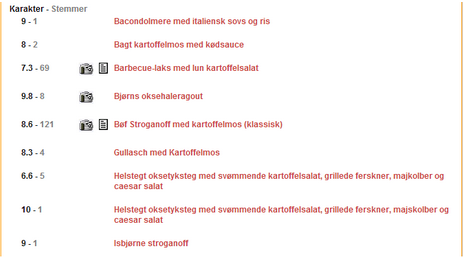
\includegraphics[scale=0.7]{billeder/forbilleder/dk-kogebogen2.png}
\capt{Liste af opskrifter, som indeholder ingredienserne Tomat, Paprika og Kartoffel.}
\label{fig:dk-kogebogen2}
\end{figure}

Brugeren vælger derefter en af opskrifterne han/hun finder mest interessant. Der er ikke overensstemmelse med, hvad \fx portionerne skal angives i. Inde på hjemmesiden er det i nogle tilfælde muligt at op- eller nedskalere portionsstørrelsen, mens der i andre tilfælde skaleres på antal personer. Derudover er der også nogle opskrifter, hvor det slet ikke er muligt at op- eller nedskalere. Her er brugeren i stedet for tvunget til selv at finde ud af, hvor stor en portion opskriften ca. passer til. Denne mangel på konsistens er endnu en af problematikkerne ved, at det er brugerne selv, som indsender opskrifterne. En endelig vurdering af DK-Kogebogen, vil kunne findes i \secref{sec:forbilleder:sammendrag}.
